
% We have demonstrated that tuning a pipline specifically for a BNS search has yieled  
% a significant improvment in sensitivity as compared to naive tunings based on a larger
% parameter space. While these are sensitive to the specific noise characteristics 
% of the detector, which will be different (broader and lower) in Advanced LIGO
% we can extrapolate that these same tuning choices will be important to revisit in the 
% first weeks of analysis. 

% I suggest also testing with sensitivites with the recolored data as well on the final
% tuning choice

\section{Introduction}
\label{sec:introduction}

The coalescence of compact binary systems are a promising source of gravitaional-wave detections from the next generation observatories, Advanced LIGO (aLIGO) and Advanced Virgo (AdV). Binary neutron star systems are likely to be one of the first sources observed by these observatories. Advanced LIGO will begin its first observing run (O1) in the fall of 2015, and will reach design sensitivity by 2018-19. Detection rate estimates for aLIGO and AdV sugest that BNS sources will be one of the most numerous source detected, with plausible
rates of $\sim 10/\mathrm{yr}$~\cite{Abadie:2010cf}. The detection of multiple BNS systems will allow us to explore the processes of stellar evolution and measure the properties of a nuetron star, including information about the nuclear equation of state\cite{lacky}.

Current electromagnetic observations suggest that the neutron star mass distribution peaks at $1.35 \Msun$--$1.5 \Msun$ with a narrow width~\cite{Kiziltan:2010ct}, although neutron stars in globular clusters seem to have a considerably wider mass distribution~\cite{Kiziltan:2010ct}. There is also evidence that a neutron star in one system has a mass as high as $\sim 3 \Msun$~\cite{Freire:2007jd}. The dimensionless spin magnitude $\chi = cJ/Gm^2$ for neutron stars is constrained by possible neutron star equations of state to a maximum of 0.7~\cite{Lo:2010bj}.  The fastest observed pulsar has a spin period of 1.4 ms~\cite{Hessels:2006ze}, corresponding to a $\chi \sim 0.4$, and the most rapidly spinning observed neutron star in a binary, J0737--3039A, has a spin of only $\chi \sim 0.05$.  

The gravitional wave from an inspiralling binary system can be separated into an inspiral portion, where the wave is slowly increasing in amplitude and frequency, a merger, and the post-merger signal. For systems with a total mass is less than $\sim 12 M_\odot$, and where the angular momenta of the compact objects is low, as is the case with BNS systems, it has been shown that post-Newtonian approximants, which model only the inspiral portion of the waveform, and are currently available at up to 3.5PN order, can provide an accurate model of the gravitational waveform for the purposes of detection.

Since we have a well-modelled gravitational wave signal, searches for gravitational waves from CBC sources use template-based matched filtering~\cite{Allen:2004gu}. The data from a detector is correlated against of bank of known template waveforms. The set of templates is chosen so that any signal will lose no more than $3\%$ of the optimal signal-to-noise ratio that would be obtained by an exactly matching template in the absence of noise. Geometric metric-based methods for placing both non-spinning and aligned spin templates have been shown to be effective for binary neutron stars~\cite{brown:2012qf}.

In addition to possible signals, and Gaussian noise, detector data contains non-Gaussian noise transients, which can generate large, spurious SNR triggers. To mitigate the effect of these noise transients, signal-consistency tests are used to create a weighted detection statistic. In addition, a signal must been seen in multiple detectors with consistent parameters. It has been shown that using a bank of templates shared between all detectors, and requiring a signal to be observed in the same template accross the detector network, improves the overall search sensitivity~\cite{samantha}. 

In this paper we present an offline search pipeline tuned for the detection of BNS sources, and show that this targeted search yields significant improvements in sensitivity to BNS sources. Whereas in prior searches for BNS systems, such as the last one conducted in S6/VSR2,3, a nonspinning template bank was constructed that contained masses up to $25M_\odot$ \cite{s6paper} and was tuned to be sensitive in all regions, we focus on soly on BNS systems with a mass range from $1-3 M_\odot$. To approximate the conditions of the first observing run with Advanced LIGO, we focus on a two-detector network composed of the Hanford (LHO) and Livingston (LLO) observatories.

This paper is organized as follows. In sec.~\ref{sec:pipeline} we describe the methodology of the search pipeline, and we present a method for estimating the significance of candidate events. In sec.~\ref{sec:tuning}, starting with the configuration suggested by \ref{samantha}, which improved upon the S6/VSR2,3 by requiring exact-match coincidence, we present a procedure for further improving the search sensitivity of the pipeline by optimizing key parameters of the search, namely the configuration of the power spectral estimation, the signal-consistency tests, the single detector SNR thresholds, and the lower frequency cutoff. 

\section{Coincident Analysis}
\label{sec:pipeline}

To search for gravitational-waves from coalescing binaries, the search pipeline implements the coincident matched-filtering algorithm proposed in \cite{samanta} A bank of post-Newtonian TaylorF2 3.5 PN order templates, generated using the metric based placement algorithm proposed in \cite{brown}, is created to span the extended binary neutron star mass range from $1-3 M\odot$. Each template, $h$, is filtered against the gravitationl-wave strain data of a detector, $s$, resulting in the matched filtering signal-to-noise ratio,

\begin{equation}
\rho (t) = \frac{(s|h)}{\sqrt{(h|h)}}.
\end{equation}

We make use of the noise-weighted inner product

\begin{equation}
(a|b) = 4 \int^{f_{nyquist}}_{f_{low}} \frac{\tilde{a}(f) \tilde{b}^*(f)} {S_n(f)} e^{2\pi i ft} df,
\end{equation}

where $\tilde{s}$ is the Fourier transform of the data, $\tilde{h}$ is the Fourier tranform of the template waveform, and $S_n(f)$ is the power spectral density (PSD).

Excursions in the SNR timeseries are recorded as single-detector triggers if they exceed a fixed SNR threshold, and are the loudest within a fixed time window of 1 second. To cope with large number of high SNR triggers caused non-Gaussian transient events, we construct a signal-based consistency test. It is a time-frequency test, constructed by splitting the template waveform in the frequency domain amoung $p$ bins that each contribute an equal amount of power. Each bin is filtered against the data to construct the matched filter output $\rho_l$. The full time-frequency $\chi^2$ is finally constructed as

\begin{equation}
\chi^2 = p \sum^p_{l=1} \left( \frac{\rho}{p} - \rho_l \right)^2.
\end{equation}

True Gravitational-wave signals, along with Gaussian-noise, return a low number for this statistic, while a noise transient, which strongly weights a limited number of bins, would return a large $\chi^2$ value. The value of this signal-consistency test along with the matched-filter SNR is used to construct the single detector detection statistic, $new SNR$, which is defined as

\begin{equation}
\rho_{new} =
  \begin{cases}
    \rho &\textrm{for } \chi^2_r \leq 1\\
    \rho[\frac{1}{2}(1+(\chi^2_r)]^{-\frac{1}{6}} &\textrm{for } \chi^2_r > 1,
  \end{cases}
\label{eq:newSNR}
\end{equation}

where $\chi^2_r$ is the reduced $\chi^2$ statistic, $\chi^2_r=\chi^2 / (2p - 2)$.

This statistic has the convenient property that for relatively quiet injections within Gaussian noise, the value is close to the simple matched-filter SNR, while also downweighting triggers caused by non-Gaussian noise.

We require that a candidate signal be present in more than one detector. In accordance with the recommendation of \cite{samantha}, we define a coincident event as a  pair of single detector triggers have the same mass and spin parameters, and are within a fixed time window of each other. This window is determined by the light-travel time between detectors, which for two-detector network of LIGO detectors we are considering is $\approx 11 ms$. The single detector new $\rho_{new}$ from the Hanford and Livingston detector, $\rho^H_{new}$ and $\rho^L_{new}$, respectively are combined into a single coincident statistic given by

\begin{equation}
\rho^c_{new} = \sqrt{(\rho^L_{new})^2 + (\rho^H_{new})^2}
\end{equation}

\subsection{Significance of Candidate Events}

In order to claim a candidate signal as a detection of a gravitational-wave, we need to determine the probability that it could have been a chance happening. We estimate the false alarm rate by forming coincidences between single detector triggers that are outside of the standard coincident time window. 

For both computational efficiency and simplicity, we choose to form background coincidences by applying a time shift to one detector. The triggers from one detector are offset by all possible non-zero integer multiples of the a fixed interval, $T_s$, for which there is coincident livetime. For this analysis we choose $T_s$ to .2 s. From all of these time slides, we collect a set of coincident triggers. As this set was formed from all of the original single detector triggers, we will refer to it as the \textit{inclusive background}, $B_{inc}$. Note, that if there is a loud gravitational-wave signal its component single detector triggers will also form coincidences that will be included within the background. The inclusive set of background triggers can be expanded as

\begin{equation}
B_{inc} = \{N_H * N_L\} \cup \{ N_H * S_L \} \cup \{S_H * N_L\},
\end{equation}

where $N_{H/L}$ are single detector noise triggers, $S_{H/L}$ are single detector triggers from gravitational-wave signals, and $\{A * B\}$ represents the set of coincidences between the single detector triggers A and B. We can define a set of background triggers that excludes coincidences, $B_{exc}$ , by excising single detector time surrounding each of the foreground coincident triggers, with components $F_H$ and $F_L$. This can be expressed as,

\begin{equation}
B_{exc} = B_{inc} - \{S_H * T_L\} - \{R_H * S_L\} - \{S_H * R_L\},
\end{equation}

where $R_{L/H} \in N_{L/H}$, and the time difference between any element in $R_{L/H}$ and any element of $F_{H/L}$ is greater than the blinding window $T_{blind}$, which in this analysis we have chosen to be 100 ms. Although the exclusive background is likely to exclude true signals, along with a set of random coincidences due to noise, a priori it cannot be determined if any given trigger belongs to the set of signal triggers or noise triggers. As such, both backgrounds are valid for different types of questions. The inclusive background admits the possibility that all triggers could be noise generated, while the exclusive background presumes that they are signal.

Given an event wih a $\rho^c_{new}=x$, we can express the false alarm rate (FAR) as

\begin{equation}
FAR_{inc/exc} (x) = N_{inc/exc} (x) / {T_B},
\end{equation}

where $N_{bkg}(x)$ is the number of coincident events in the estimated background with a $\rho^c_{new} > x$. $T_F$ is the coincident livetime, the cumulative amount of time in which both detectors of the two-detector network is active. $T_B$ refers to the effective background time, which can be accurately estimated from the single-detector livetimes $T_H$ and $T_L$ for the Hanford and Livingston detectors, respectively, as

\begin{eqnarray}
T_B =  T_H * T_H / T_s
\end{eqnarray}

Note, that this is not an exact calculation of the background livetime, which can be obtained by explicitly calculating the amount of overlapping time between the two ifos for each time slide and taking the sum. Notice, that the estimate is equivelant to the exact calculation, when the start and end of chunck of analyzed data lies on multiple of the timslide interval. As such, we can calculate the upper bound on the difference between the true and estimated value of the background livetime as

\begin{eqnarray}
ERROR < 2 * N_{chunks} * T_s,
\end{eqnarray}

where $N_{chunks}$ is the number of non-contigious analysis chunks.

As our analysis discards chunks of data that are less than 2048 seconds in length, and  $T_s=200$ ms, the relative error is strictly less than $.02\%$, and so can safely be considered negligible.



\section{Optimizing Search Sensitivity}
\label{sec:tuning}

In this section, we retune several parameters of a CBC search, with the aim of creating a sensitive search for Binary Neutron star sources. The potential parameter space of tuning choices is quite large, so we have started with the settings that mimic the lowmass CBC search performed in S6/VSR23. 

In this section, we describe the procedure for evaluating the search perfornance of a particular set of tuning parameters. The metric we will use for evaluation is sensitvity volume of the search integrated over the coincident livetime, $VT$, which can be expressed as,

\begin{eqnarray}
VT (F) = \int \epsilon(F;r,\Omega,\Lambda, t)p(r,\Omega,\Lambda)r^2 dr d\Omega dt
\end{eqnarray}

The quanitity VT is directly proportional to the expected number of detected gravitaional-wave signals.

In the subsequent sections, we will use this metric to evaluate potential options for tuning the PSD estimation, and chisq binning.

To assess the performance of a given set of tunings, we evalute VT for 3 one-week time spans of S6 data. 

% Heavily reference account of method as in cbc_ahope_paper (in preparation)

\subsection{Power Spectrum Estimation}
\label{sec:psd}

Because the overall sensitivity of a detector along with the shape of its power spectral density (PSD) changes over time, the spectral density used to calculated the SNR of candidate events is periodically recalculated. The S6/VSR2,3 analysis recomputed the PSD using every 1920 seconds. However, due to the additional padding required for filtering, 2048s of data was used for each PSD estimate. Each 2048s chunk of data is subdivided into 15 segments, each with 256s duration and overlapped by 50$\%$. The PSD each chunk is calculated by first taking the median average of the Fourier transform of each segment. Finally, we truncate the inverse of the PSD in the time domain to restrict the filter corruption to a fixed length of time. In addition, this has the effect of smoothing out lines within the spectrum. An inverse truncation value of 16 seconds was used throughout S6/VSR2,3. 

We investigate a straightforward improvement to this algorithm. Instead of calculating the PSD using 256 second segments and applying a 16 second inverse spectrum truncation, we propose calculating the PSD using 16 second segments directly, interpolating for the intended use case, and finally applying the same 16s inverse spectrum truncation. The results of this investigation are shown in figure Fig.~\ref{fig:psd}, where the sensitive volume-time is compared for the initial reference configuration and for the proposed configuration as a function of the inverse false alarm rate. The proposed PSD estimation shows clear improvement over the initial method, resulting in an average $\approx 18\%$ increase in sensitivity between inverse false alarm rates of $10^3$ and $10^4$ years.

%In this section, we investigate a straightforward improvement to the estimation of PSDs %within the search pipeline.

%This value is chosen to be as small as possible to limit the amount of data removed due to filter startup time, but large enough so that the PSD estimate itself can capture the complex behavior of the numerous frequency lines. For S6 data this was chosen to be 16 seconds. Due to technical limitations, not scientific ones, the length of the PSD estimate was chosen to be 256 seconds. 

%Using a newer pipeline that has removed these limitations, we investigate the benefit of directly measure the PSD in 16 second intervals, given that this satisfies the same constraint on correlation length. The allows an increased number of PSD estimates from 15 to ~250, which has a impact on the variance of the PSD estimate. (how much??). 

\begin{figure}
\centering
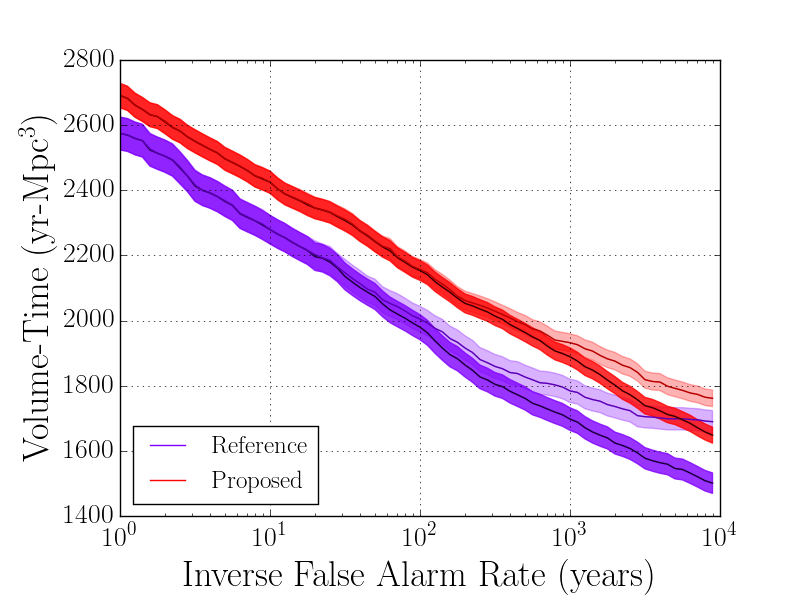
\includegraphics[width=0.5\textwidth]{papers/bns_o1_dev/figures/psd_combined.png}
\caption{\label{fig:psd} 
The combined VT as a function of inverse false alarm rate, for the combined three weeks of analysis, and for an injection population that uniformly covers the parameter space of the non-spinning BNS region, with component masses between $1- 3M_\odot$. Darker colored lines indicate the inclusive IFAR value, while lighter lines show the exclusive IFAR. The reference (red) PSD estimation uses 15, 256s segments. The proposed (purple) tuning which uses 252, 16s segments. Both truncate the inverse spectrum in the time domain to 16 seconds. The proposed configuration improves the search sensitivity by $\approx 18\% $ at a false alarm rate of 1 per 1000 years.
}
\end{figure}

\subsection{Signal-to-noise Threshold}
\label{sec:snr}

For each detector, triggers are recorded when the signal-to-noise ratio exceeds a pre-determined threshold, $\rho_t$. For the S6/VSR2,3 CBC search, only triggers with an SNR above 5.5 were recorded. Beginning with the PSD tunings proposed in sec.~\ref{sec:psd}, we investigate the effect of lowering the SNR threshold to 5.0. A comparison of the search sensitivity at $\rho_t=5.5$ and $\rho_t=5.0$ is shown in Fig.~\ref{fig:snrthreshold}. We see that lowering $\rho_t$ from 5.5 to 5.0 has not resulted in a significant improvement in sensitivity. We observe that at high inverse false alarm rate, the inclusive IFAR is identical between the two thresholds, but that there is a very minor increase in sensitivity when using the exclusive IFAR.

In fig.~\ref{fig:ifarifar} we explore where the differences between the inclusive and exclusive IFAR estimates are the greatest. At a fixed exclusive IFAR, which is directly proportional to the combined NewSNR of an injection trigger, we find that there is an inverse relation between the inclusive IFAR and the minimum single detector SNR. This indicates that lowering the SNR threshold below $\approx 5.3$ will not yield an improvement in sensitivity at inclusieve false alarm rate of 1 in 1000 years, for a two-detector search composed of the Hanford and Livingston LIGO observatories. Note that this result cannot be generalized to a multi-detector network, where there can be a non-trivial increase in detection confidence due to the presence of quiet trigger in the additional detectors. Further work is required to characterize the appropriate SNR thresholds for multi-detector networks.

%maybe add ranking stat to the right axis of this plot?


\begin{figure}
\centering
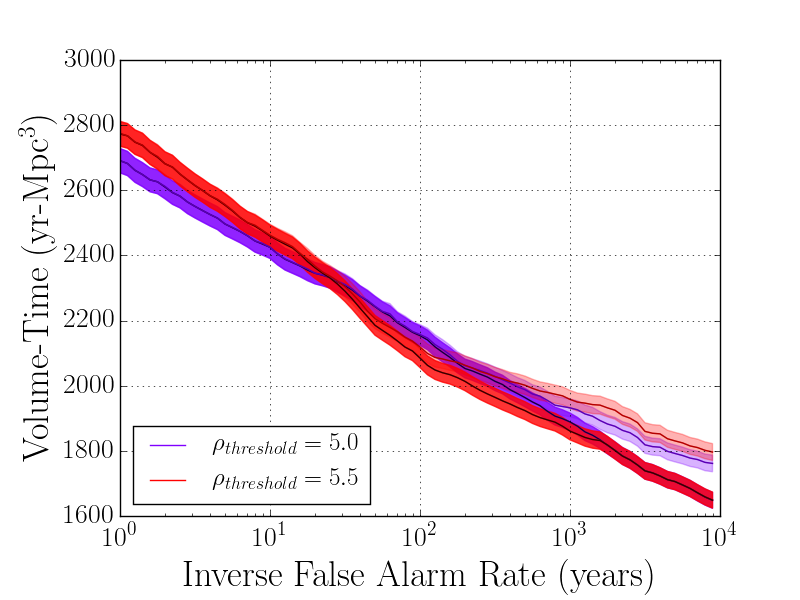
\includegraphics[width=0.5\textwidth]{papers/bns_o1_dev/figures/snr_combined.png}
\caption{\label{fig:snrthreshold} 
The combined VT as a function of inverse false alarm rate, for the combined three weeks of analysis, and for an injection population that uniformly covers the parameter space of the non-spinning BNS region, with component masses between $1- 3M_\odot$. Darker colored lines indicate the inclusive IFAR value, while lighter lines show the exclusive IFAR. 
}
\end{figure}

\begin{figure}
\centering
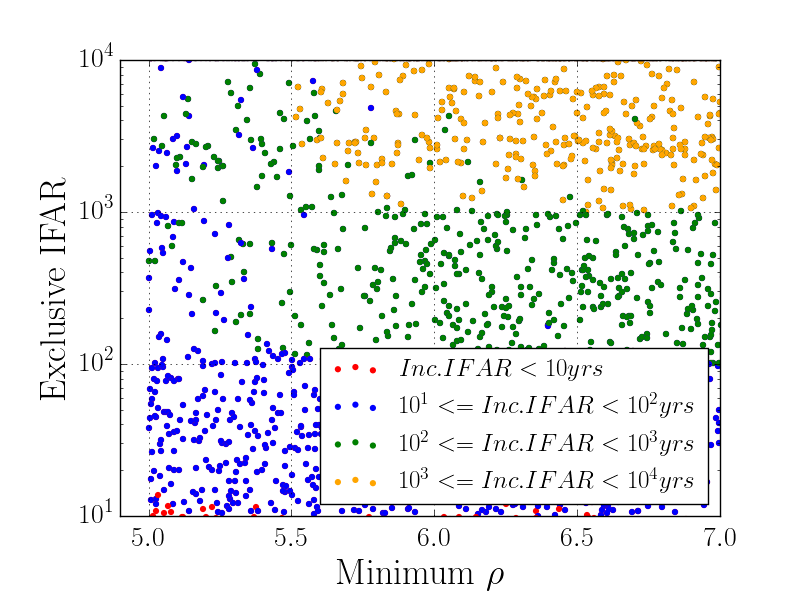
\includegraphics[width=0.5\textwidth]{papers/bns_o1_dev/figures/ifarifar.png}
\caption{\label{fig:ifarifar} 
The distribution of Exclusive IFAR as a function of the minumum single detector SNR, for an injection population that uniformly covers the parameter space of the non-spinning BNS region, with component masses between $1- 3M_\odot$. Injections are colored by the value of their inclusive IFAR. We observe that there is an inverse relationship between the inclusive IFAR and the minimum SNR value. This indicates that for a given value of inclusive IFAR, there is a corresponding SNR threshold, below which, the search sensitivity as function of inclusive IFAR will not improve
}
\end{figure}


\subsection{Signal-consistency Test and Ranking Statistic}

As detailed in sec.~\ref{sec:pipeline}, the single-detector ranking statistic, $\rho_{new}$, is the SNR weighted by the time-frequency consistency test. The time-frequency signal consistancy test breaks a template into $p$ bins of each power. Although the boundaries of the bins are defined in the frequency domain, as the template is a monotonic function of time and frequency, we can outline the rough time-frequency boundaries of each bin as demonstrated in fig~\ref{fig:chisqbins}, for the 16 bins used in the S6/VSR2,3 analysis. Since the response of the time-frequency chisq is dependent on the morphology of the non-guassian noise present in the data, we investigate if increasing the number of time-frequency bins for a BNS focused search, where the average template duration is significantly longer than for searches that include higher mass templates, has an effect on the search sensitivity.

Starting with the analysis tunings suggested in \ref{sec:snr}, we compare the search sensitivity at a fixed exclusive FAR of 1/1000 years. The results in Fig.~\ref{fig:vbin}, show that increasing the number of time-frequency bins from 16 to 64-256 there is an $\approx 12\%$ improvement in search sensitivity. From the results of Fig~.\ref{fig:fchisq} we see  that this improvement occurs at all values of the FAR.

%The primary ranking statistic we use is "NewSNR". It is a chisq-weighted SNR defined as, INSERT DEFINITION. It has the interesting behavior that at lowSNR values, it is very close numerically to the standard SNR. The chisq chops of the template waveform into bins of equal contribution to the SNR for real signals. For each bin and partial matchedfilter in calculated, and the difference between this value and fraction of the expected fraction of the total SNR gives the chisq statistic. This can be expressed as , INSERT DEFINITION, where is the number of bins. 



%The key tunable parameter in this statistic is the number of chisq bins that one choses to use. In S6 , 16 chisq bins wer used in the "lowmass" search which covered a much larger range than we are focued in this study on tuning for. Due to the expected nature of at least a known subset of glitches, it is expected that this parameter can be optimized differently for different mass regions. In particular if the characteristic time frequency space of a given glitch is not wholely contained within a given bin, than the statistic can be improved by using larger bins. In general, the best separation from noise occurs in the case where the bin sizes are approximately the same as most glitches. Due to the varied nature of glitches however, and the possibility for extremely rare (one-off) glitch types, a straightforward method for testing for an optimal value is to simply perform the empirical analysis.


\begin{figure}
\centering
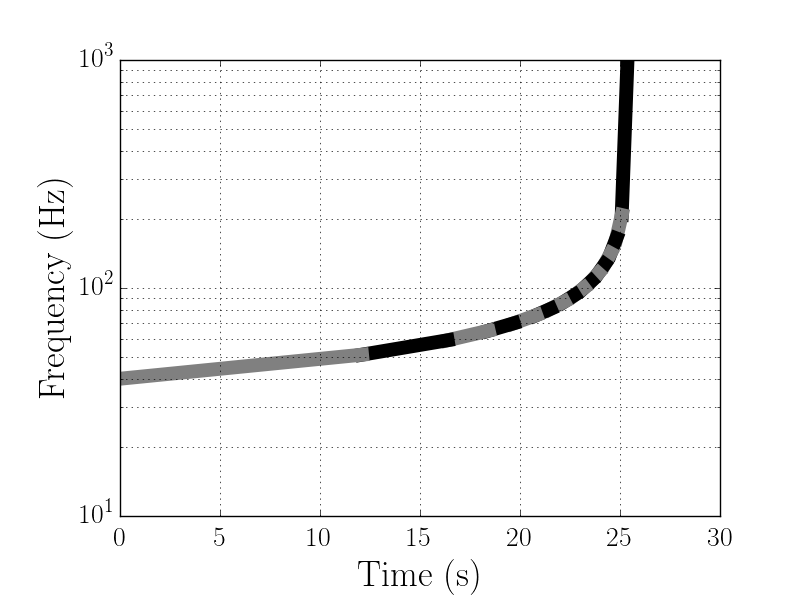
\includegraphics[width=0.5\textwidth]{papers/bns_o1_dev/figures/bin.png}
\caption{\label{fig:chisqbins} 
Approximate boundaries of the 16 bins that make up the time-frequency signal consistency test, as used in S6/VSR2,3, overlaid on the track of a $1.4-1.4M_odot$ BNS waveform. 
}
\end{figure}

\begin{figure}
\centering
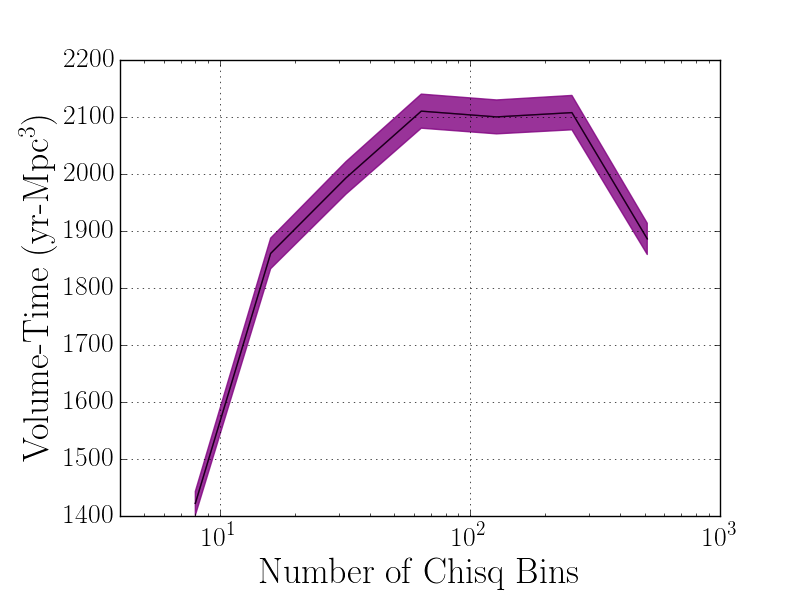
\includegraphics[width=0.5\textwidth]{papers/bns_o1_dev/figures/cb.png}
\caption{\label{fig:vbin} 
The combined VT at inclusive inverse false alarm rate of 1/1000 years as a function of the number of time-frequency bins in the signal-consistency test, for the combined three weeks of analysis, and for an injection population that uniformly covers the parameter space of the non-spinning BNS region, with component masses between $1- 3M_\odot$. There is an $\approx 13\% $ improvement in the analysis sensitivity when using 64-256 bins, as compared to the reference 16 bins.
}
\end{figure}

\begin{figure}
\centering
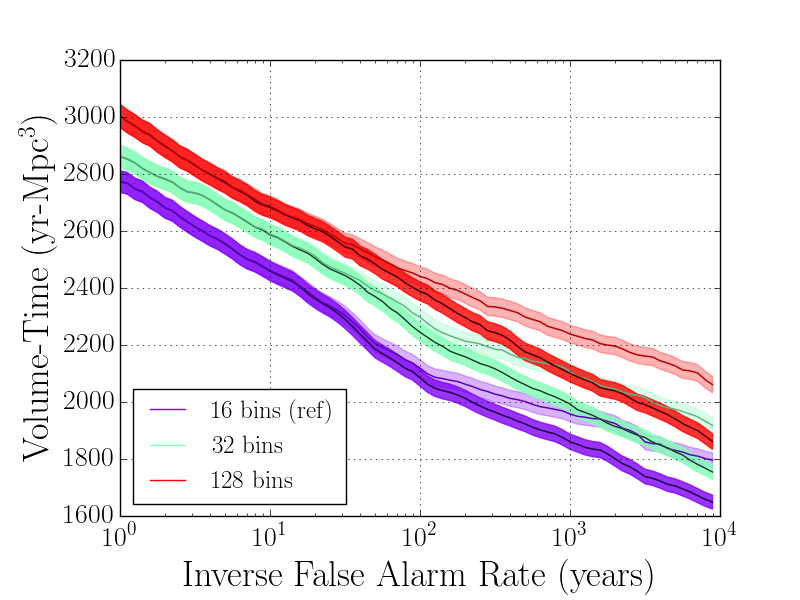
\includegraphics[width=0.5\textwidth]{papers/bns_o1_dev/figures/chisq_combined.png}
\caption{\label{fig:fchisq} 
The combined VT as a function of inverse false alarm rate, for the combined three weeks of analysis, and for an injection population that uniformly covers the parameter space of the non-spinning BNS region, with component masses between $1- 3M_\odot$. Darker colored lines indicate the inclusive IFAR value, while lighter lines show the exclusive IFAR. 
}
\end{figure}

\subsection{Lower-frequency cutoff of the matched filter}

As we have been using S6 LIGO data in the previous sectons, and expect that seismic noise will dominate at low frequencies, we have used the same 40Hz lower-frequency cutoff used in the S6/VSR2,3 analysis. We can verify that using a 40Hz lower-frequency cutoff does not impact search peformance by constructing

\begin{equation}
V(f_{low}) = \left[ \frac{\int_{f_{low}} \frac{h^{*}(f)h(f)}{S_n(f)} df}{\int_{0} \frac{h^*(f)h(f)}{S_n(f)} df} \right]^3
\end{equation}

where $h(f)$ is a template waveform, $S_n(f)$ is the power spectral densitity, and the quantity $V(f_{low})$ represents the fraction of the optimal volume for a single template
filtered from the lower-frequency cutoff, $f_{low}$. Fig~\ref{fig:flow} shows that filtering from 40Hz only results in only a $1\%$ loss in search volume, for a single 1.4-1.4$M_\odot$ TaylorF2 template. 

%The initial ligo noise curves do not caontain significant power below 40Hz for CBC signals, as we progress towards ZDHP, however this will change, and we will need to begin searching with template that begin at a lower frequency. This also implies that they will be longer, and whereas from 40Hz the longest template in our bank which is a 1-1 system was 48s long, it is 95s from 30Hz and 600s from 15 Hz. For O1, we expect that there may be additional power that is worth filtering below 40Hz, however, the increase in correlation length means that there is an increased chance of a filter overlapping a non-gaussian noise event (glitch) that will impact the filter performance. 

%As such, in the case of non-gaussian noise, there is a trade-off between the increased SNR recovery and the increased chance of glitch overlap. If we model this problablity as linearly proportional to the length of the template it can be expressed as, INSERT DEFINITION.


\begin{figure}
\centering
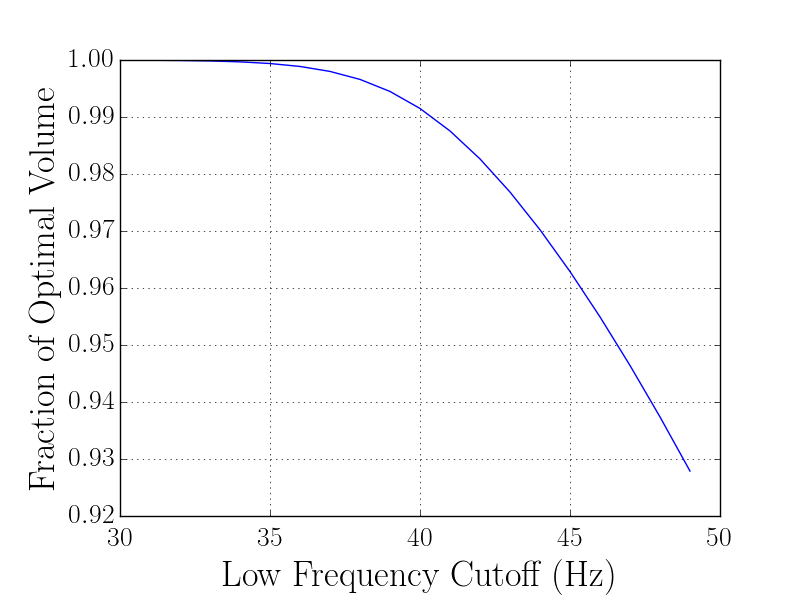
\includegraphics[width=0.5\textwidth]{papers/bns_o1_dev/figures/flow.png}
\caption{\label{fig:flow} 
The fraction of the optimal search volume for a $1.4-1.4 M_\odot$ TaylorF2 BNS waveform, as a function of the lower-frequency cutoff of the matched filter. 
}
\end{figure}

%\subsection{False Alarm Rate vs. Parameter space coverage}
% include for Gaussian noise, S6, and recolored S6 data, % no injection analysis here

\section{Sensitivity to Astrophysical Sources}
\subsection{Nonpinning injections}

In this section we test the sensitivity to a broad mass distribution ($1-3 \M_\odot$) of sources where the component neutron stars are non-spinning. The parameter space corresponds to the intended coverage of the non-spinning template bank we have tuned against in \ref{sec:tuning}.  If \ref{fig:nonspin} we show the reference and tuned pipeline configuration using both the aligned spin, and non-spinning template banks. We see that for either template bank there is a ~25$\%$ increase in search volume using the improved pipeline tunings. Both template banks use the same gemetric placement algorithm and required minimal match, and since the injection set is strictly within the boundaries of both template banks, the loss of $\approx 6\%$ loss in search volume when using the aligned spin template bank is due to the increase in background.

\begin{figure}
\centering
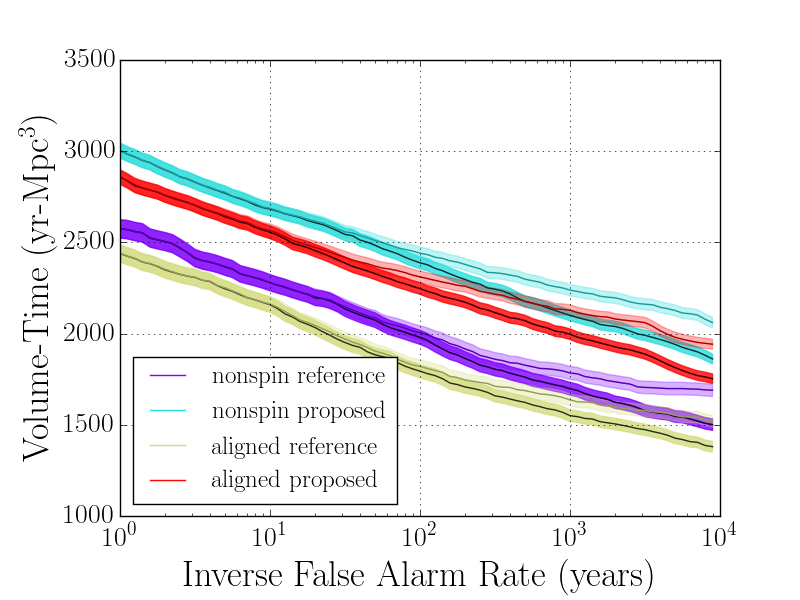
\includegraphics[width=0.5\textwidth]{papers/bns_o1_dev/figures/ns_combined.png}
\caption{\label{fig:nonspin} 
The combined VT as a function of inverse false alarm rate, for the
three sample analysis weeks, for an injection population that uniformly covers parameter space of the non-spinning BNS region, $1- 3M_\odot$. For both the non-spinning template bank and the aligned spin template bank there is $\approx 25 \%$ improvement in search sensitivity.
}
\end{figure}

\subsection{Astrophysical Source Distribution}

We test the focused BNS search's sensitivity to an estimate of astrophysical sources using an injection population drawn from a conservative range of mass and spin distributions. We clearly see in \ref{fig:rest} that a search using only a non-spinning template bank yields a $\approx{7\%}$ improvment in search sensitvity over one that covers an expansive spin range. If the true distribution of signals matches the expectations from current observations, then a non-spinning template bank is the preferred options. Note, that future work should investigate alternate possibilities for incorporating expected population distributions into the search directly, wich may allow a more fine-grained inclusion of spinning regions of the parameter space while sacrificing less in overall sensitivity to the most likely signals.

\begin{figure}
\centering
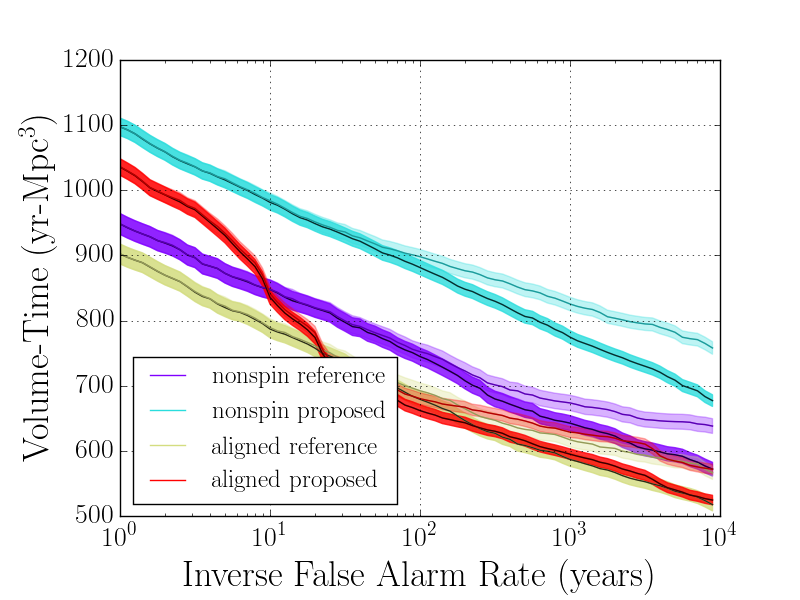
\includegraphics[width=0.5\textwidth]{papers/bns_o1_dev/figures/rest_combined.png}
\caption{\label{fig:rest} 
The VT as a function of inverse false alarm rate, for the
three sample analysis weeks, for a conservative mass and spin distribution. There is an $\approx 7\%$ drop in sensitivity when using the full aligned spin template bank when compared to the the non-spinning
template bank.}
\end{figure}

\subsection{Aligned Spin Sources}

In this section we choose a distribution of sources drawn unformly from the parameter space that the aligned spin template bank is intended to cover. As one would expected, this distribution should be more favourable to the aligned spin template bank than the non-spinning one. We find in \ref{fig:aligned} that although the aligned spin template only provides a marginal $\approx 2\%$ improvement in search volume, which we note is close to the measured statistical error. 

\begin{figure}
\centering
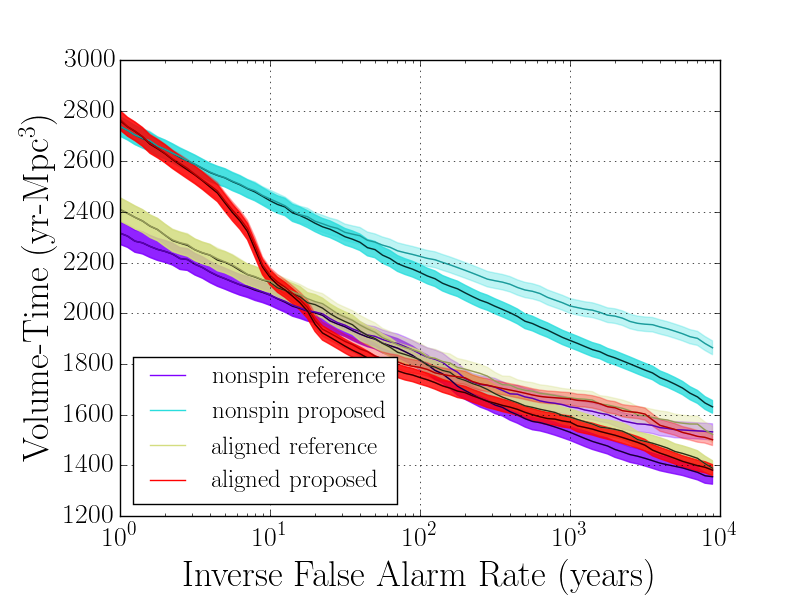
\includegraphics[width=0.5\textwidth]{papers/bns_o1_dev/figures/aligned_combined.png}
\caption{\label{fig:aligned} 
The combined VT as a function of inverse false alarm rate, for the
three sample analysis weeks, for an injection population that uniformly covers parameter space of the aligned spinning BNS region, $1- 3M_\odot$, and $|\chi| <= 0.4$. At a false alarm rate of 1 per 1000 years, the aligned spin template bank improves the overall search sensitivity by only $\approx 2\%$
}
\end{figure}

\subsection{Precessing Sources}

As in practice we do not expect that coalescing systems will preferentially contain binary neutron stars whose spin is aligned with the orbital angular memoment, we also test a population of isotropically distribution angles over the full mass and spin magnitudes. This will allow the systms to precess, however, as the mass ratio of a BNS systems and the magnitude of the spin is small the effect of precession is not significant. Although the injection population covers the full range of spin magnitudes, which the algined spin template bank is designed to recover, the nonspinning template bank is marginally more sensitive,  fig.\ref{fig:prec} shows there is an $\approx 1.5\%$ increase in search volume. A source population that is highly weighted towards higly spinning systems would be required for the aligned spin template to substantially improve the search sensitivity over the nonspinning template bank. 

\begin{figure}
\centering
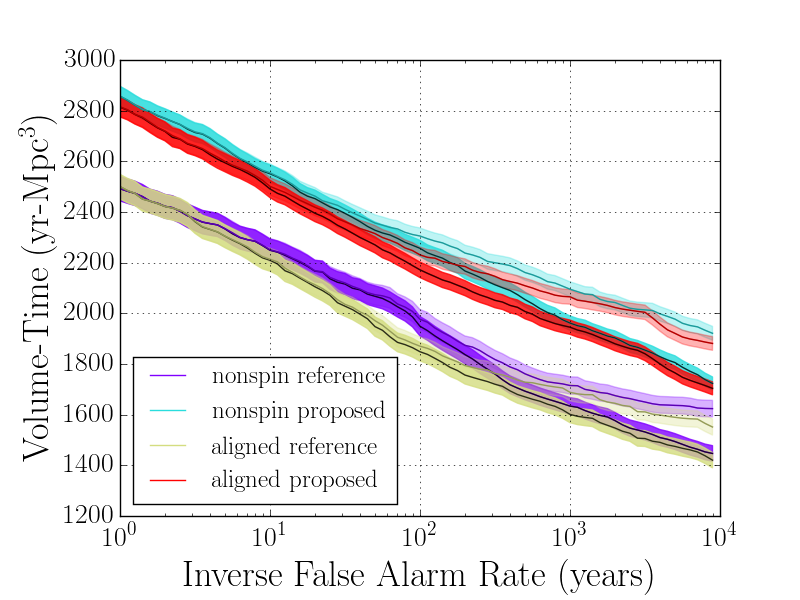
\includegraphics[width=0.5\textwidth]{papers/bns_o1_dev/figures/prec_combined.png}
\caption{\label{fig:prec} 
The combined volume - time product as a function of inverse false alarm rate, for the
three sample analysis weeks, for an injection population that uniformly covers parameter space of the non-spinning BNS region, $1- 3M_\odot$. 
}
\end{figure}



% comment on the high alinged spin case, where we can place templates

\section{Conclusions}
\label{sec:conclusions}
